\documentclass{article}
\usepackage{fancyhdr}
\usepackage{graphicx}
\usepackage{hyperref}
\usepackage{booktabs}
\usepackage{array}
\usepackage{amsmath}
\usepackage[table]{xcolor}
\usepackage{xcolor}
\usepackage{longtable}
\usepackage[a4paper, margin=1in]{geometry}
\usepackage{caption}
\usepackage{ulem}















\pagestyle{fancy}
\fancyhead[L]{Cahier des Charges Technique : \textit{An Era of the Seas}}
\fancyfoot[L]{Dream Chasers}
\fancyfoot[C]{
    \begin{minipage}{1.5cm}
        \centering
        
\includegraphics[width=1cm]{logo.png}
    \end{minipage}
}
\fancyfoot[R]{\thepage}

\renewcommand{\footrulewidth}{0.1pt}
\renewcommand{\sectionmark}[1]{}
\renewcommand{\subsectionmark}[1]{}
\renewcommand{\contentsname}{}

\definecolor{lightblue}{HTML}{55FFFF}
\definecolor{pastelblue}{HTML}{097CA5}















\title{\textbf{Cahier des Charges Technique}\\
\textbf{\textit{An Era of the Seas}}}
\author{
    \begin{minipage}[c]{\textwidth}
        \centering
        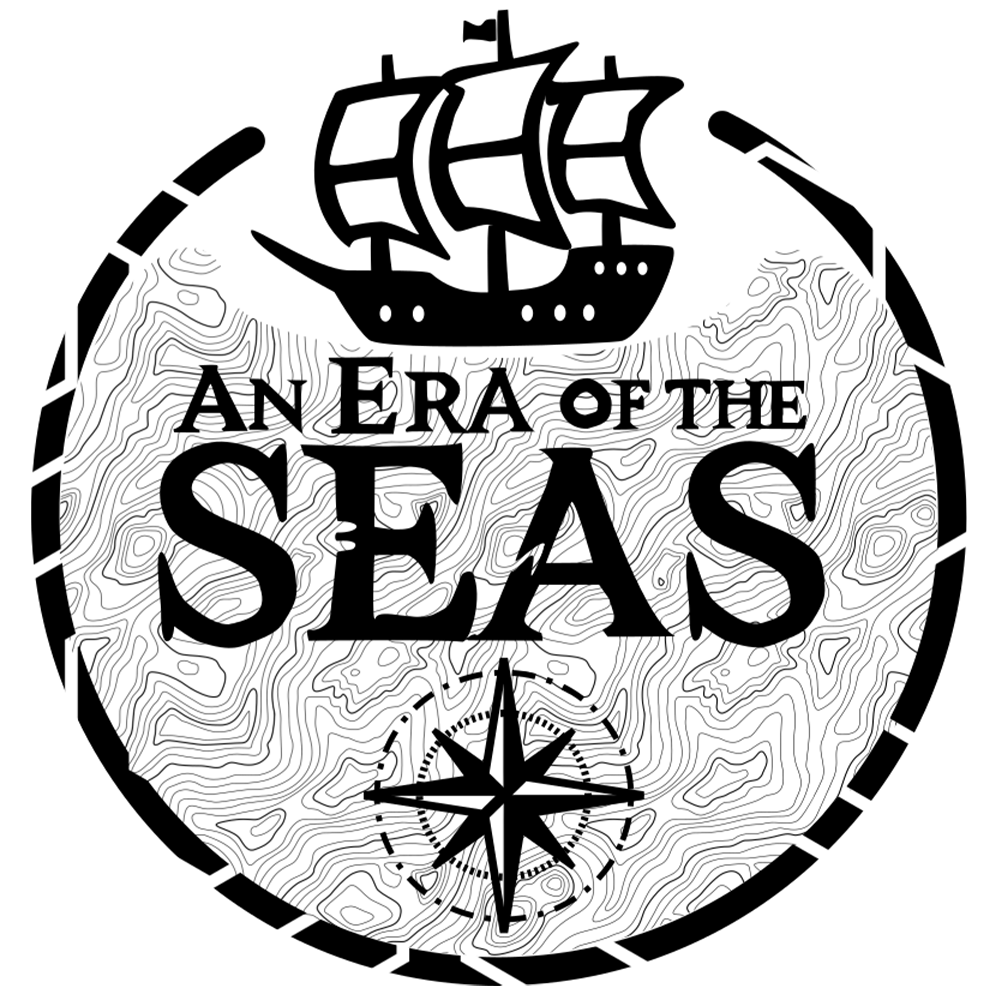
\includegraphics[width=3.5in]{AEotS Logo.png} \\
        \vspace{2cm}
        
\includegraphics[width=4in]{logo text.png}
    \end{minipage}
}
\date{}















\begin{document}

\maketitle

\vfill
\begin{center}
    \textbf{Lin Jérôme}\\
    \textbf{Ben Abdallah Achref}\\
    \textbf{Bruno Ethan}\\
    \textbf{Devin Joseph}\\
    \textbf{Classe : A1}
\end{center}















\newpage
\thispagestyle{empty}
\addtocounter{page}{-1}
\null















\newpage
\begin{table}[h]
    \centering
    \begin{tabular}{|>{\columncolor{pastelblue!60}}l|c|c|c|c|}
        \hline
        \rowcolor{pastelblue!60}
        \textbf{Tâhes} & \textbf{Jérôme} & \textbf{Achref} & \textbf{Ethan} & \textbf{Joseph}\\
        \hline
        Menu \& UI & \cellcolor{blue}R &  & \cellcolor{cyan}S &\\
        \hline
        Simulation de l'eau & & & \cellcolor{blue}R & \cellcolor{cyan}S\\
        \hline
        Simulation de la météo & & \cellcolor{blue}R & \cellcolor{cyan}S &\\
        \hline
        Mouvements (bateau, joueur...) & & & \cellcolor{cyan}S & \cellcolor{blue}R\\
        \hline
        Mouvements IA (ennemis, mouvements, attaques) & & \cellcolor{blue}R & & \cellcolor{cyan}S\\
        \hline
        Carte & \cellcolor{cyan}S & & \cellcolor{blue}R &\\
        \hline
        Système de localisation (carte, bousole...) & & \cellcolor{cyan}S & & \cellcolor{blue}R\\
        \hline
        Statistiques des objets & \cellcolor{blue}R & & & \cellcolor{cyan}S\\
        \hline
        Système de pêche & \cellcolor{cyan}S & \cellcolor{blue}R & &\\
        \hline
        Système de faim & & \cellcolor{cyan}S & \cellcolor{blue}R &\\
        \hline
        Réseau & \cellcolor{blue}R & \cellcolor{cyan}S & &\\
        \hline
        Multijoueur & \cellcolor{cyan}S & & & \cellcolor{blue}R\\
        \hline
        Histoire(Lore) & & & \cellcolor{cyan}S & \cellcolor{blue}R\\
        \hline
        Quêtes & & \cellcolor{cyan}S & \cellcolor{blue}R &\\
        \hline
        Site Web & & \cellcolor{blue}R & & \cellcolor{cyan}S\\
        \hline
        Design des entités & & \cellcolor{blue}R & \cellcolor{cyan}S &\\
        \hline
        Animations des entités & \cellcolor{cyan}S & & \cellcolor{blue}R &\\
        \hline
        SFX & \cellcolor{blue}R & & & \cellcolor{cyan}S\\
        \hline
        Musiques & \cellcolor{blue}R & \cellcolor{cyan}S & &\\
        \hline
        Optimisation du code & \cellcolor{blue}R & \cellcolor{blue}S & \cellcolor{blue}S & \cellcolor{blue}S\\
        \hline
        Correction de la langue & \cellcolor{cyan}S & & & \cellcolor{blue}R\\
        \hline
        Tests & \cellcolor{blue}R & \cellcolor{blue}R & \cellcolor{blue}R & \cellcolor{blue}R\\
        \hline
    \end{tabular}
\end{table}

\begin{itemize}
    \item \textcolor{blue}{R : Responsable}
    \item \textcolor{cyan}{S : Supléant}
\end{itemize}

















\newpage

\begin{itemize}
    \item Nom du groupe : Dream Chasers
    \item Nom du projet : \textit{An Era of the Seas}
\end{itemize}





\begin{longtable}{|l|l|l|c|}
    \caption*{\textbf{\uline{Noms des membres}}}\\
    \hline
    \rowcolor{pastelblue!60}
    Nom & Prénoms & Login & Classe\\
    \hline
    Ben Abdallah & Achref & achref.ben-abdallah & A1\\
    \hline
    Bruno & Ethan & ethan.bruno & A1\\
    \hline
    Devin & Joseph & joseph.devin & A1\\
    \hline
    Lin & Jérôme & jerome.lin & A1\\
    \hline
\end{longtable}





\begin{longtable}{|c|c|c|c|c|}
    \caption*{\textbf{\uline{Type de jeu}}}\\
    \hline
    \cellcolor{lightblue}Action/Aventure & Battle Royale & Beat them all & Combat & Simulation\\
    \hline
    \cellcolor{lightblue}FPS & MMORPG & MOBA & Party Games & Survival Horror\\
    \hline
    Plateforme & Puzzles & Reflexion & Rogue Like & TPS\\
    \hline
    \cellcolor{lightblue}RPG & RTS & Sandbox & Shoot them up & Course\\
    \hline
    Autre : & \multicolumn{4}{|c|}{}\\
    \hline
\end{longtable}





\begin{longtable}{|>{\columncolor{pastelblue!60}}l|l|l|l|l|}
    \caption*{\textbf{\uline{Caractéristiques}}}\\
    \hline
    \multicolumn{5}{|c|}{\cellcolor{pastelblue!60}\textbf{Caractéristiques générales du jeu}}\\
    \hline
    IA & \cellcolor{lightblue}Errer & \cellcolor{lightblue}Attaquer & \cellcolor{lightblue}S'échapper & "Path Finder"\\
    \hline
    Multijoueur & \cellcolor{lightblue}Coopératif & Battle (2-4) & \multicolumn{2}{|l|}{Massif}\\
    \hline
    Réseau & P2P & Lan & \multicolumn{2}{|l|}{\cellcolor{lightblue}Online}\\
    \hline
    \multicolumn{5}{|c|}{\cellcolor{pastelblue!60}\textbf{Caractéristiques graphiques}}\\
    \hline
    Dimension & 2D & \cellcolor{lightblue}3D & Autres : &\\
    \hline
    Particularités & Stéreoscopie & AR & \multicolumn{2}{|l|}{VR}\\
    \hline
    Graphiques & \cellcolor{lightblue}Perso & Custom & \multicolumn{2}{|l|}{\cellcolor{lightblue}Existant}\\
    \hline
    Précisions : & \multicolumn{4}{|c|}{}\\
    \hline
    \multicolumn{5}{|c|}{\cellcolor{pastelblue!60}\textbf{Caractéristiques sonores}}\\
    \hline
    Musique & Perso & Custom & \multicolumn{2}{|l|}{\cellcolor{lightblue}Existant}\\
    \hline
    FX & Perso & \cellcolor{lightblue}Custom & \multicolumn{2}{|l|}{Existant}\\
    \hline
    Précisions : & \multicolumn{4}{|c|}{Thème musicale orienté vers l'univers maritime}\\
    \hline
    \multicolumn{5}{|c|}{\cellcolor{pastelblue!60}\textbf{Autres caractéristiques}}\\
    \hline
    Site Web & Perso & \cellcolor{lightblue}Custom & \multicolumn{2}{|l|}{Préfabriqué}\\
    \hline
\end{longtable}







\begin{figure}[h]
    \caption*{\textbf{\uline{Diagramme de GANTT}}}
    \centering
    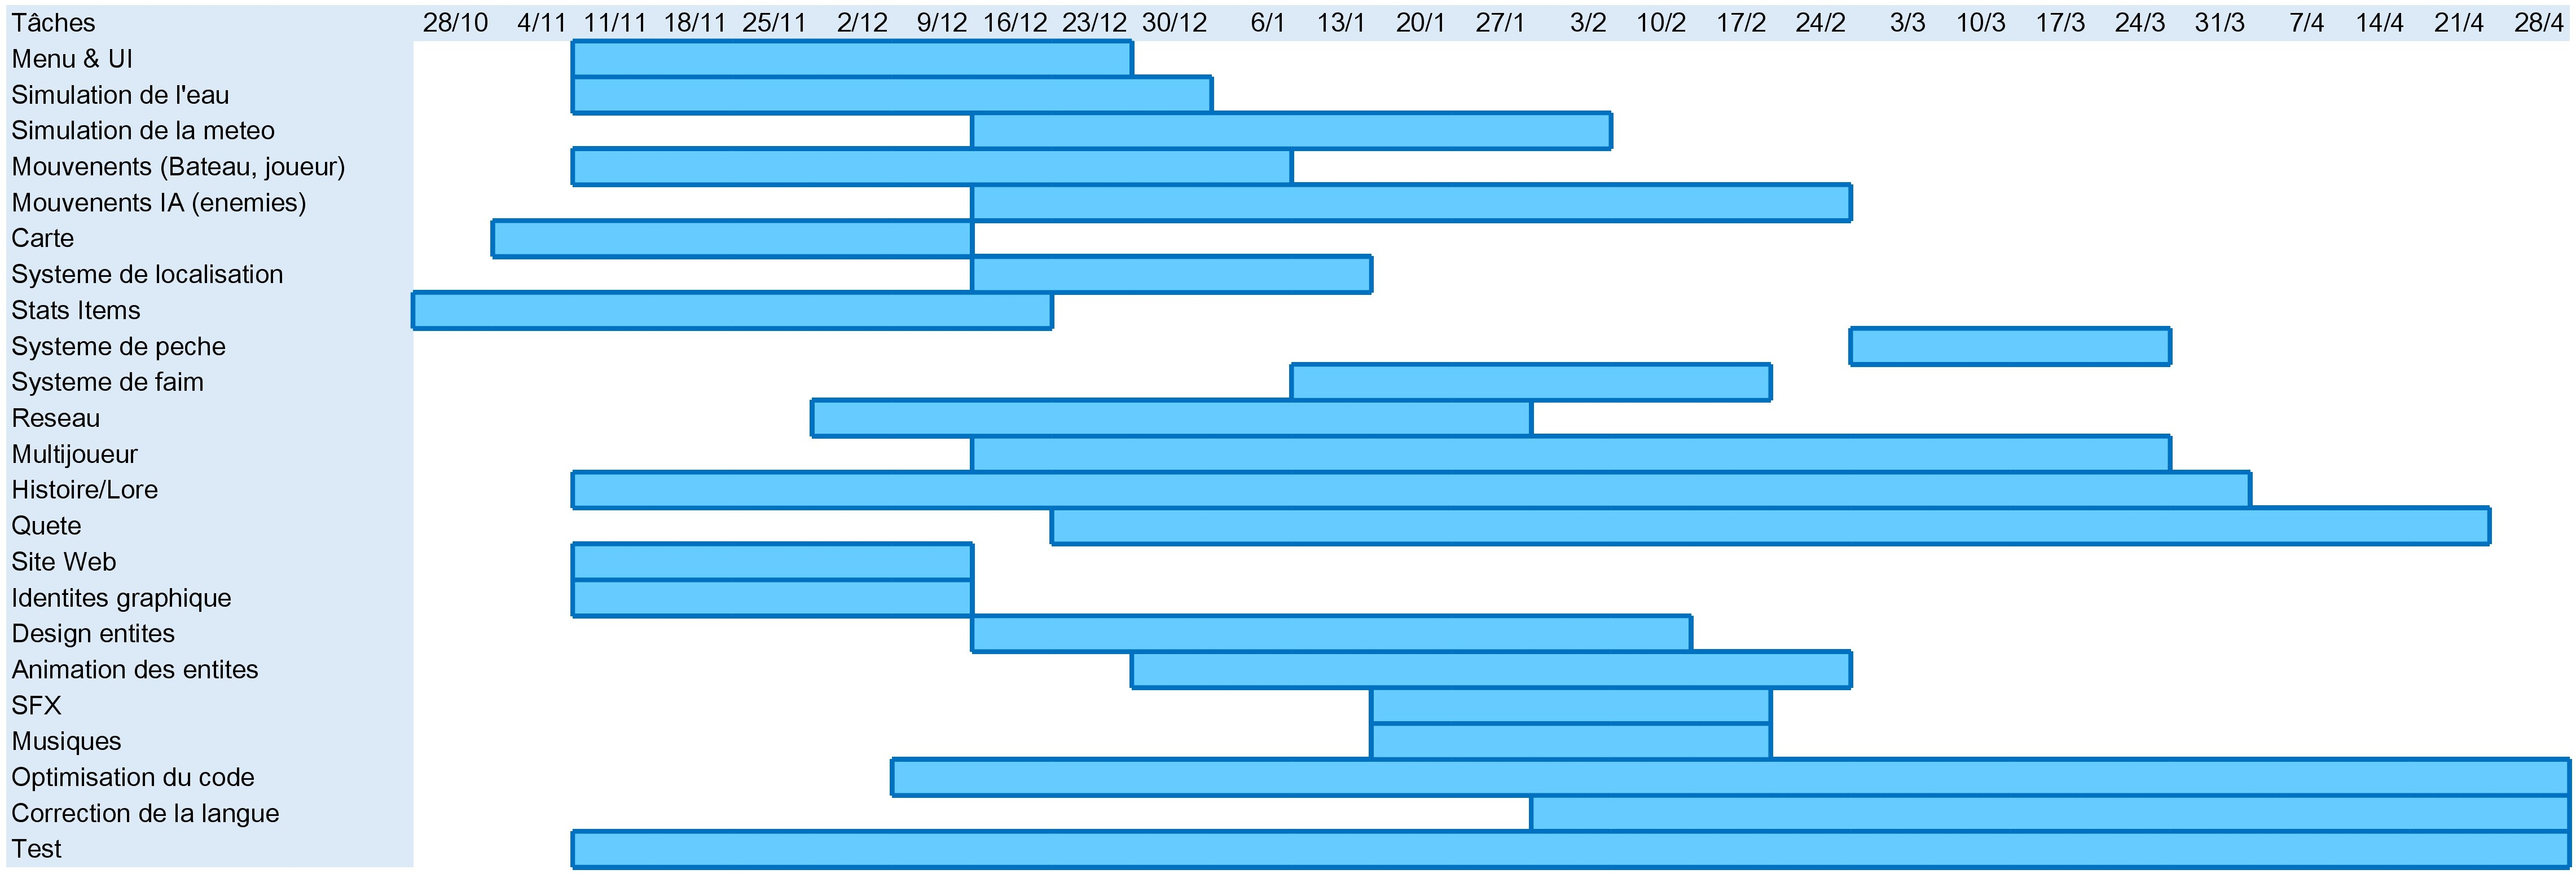
\includegraphics[angle=90, width=3.22in]{gant.png}
    \label{fig:mon_image}
\end{figure}









\end{document}